%% LyX 2.1.4 created this file.  For more info, see http://www.lyx.org/.
%% Do not edit unless you really know what you are doing.
\documentclass[english]{article}
\usepackage[T1]{fontenc}
\usepackage[latin9]{inputenc}
\usepackage{geometry}
\geometry{verbose,tmargin=3cm,bmargin=3cm,lmargin=3cm,rmargin=3cm}
\usepackage{color}
\usepackage{babel}
\usepackage{float}
\usepackage{textcomp}
\usepackage{amsmath}
\usepackage{amsthm}
\usepackage{graphicx}
\usepackage[unicode=true,pdfusetitle,
 bookmarks=true,bookmarksnumbered=true,bookmarksopen=true,bookmarksopenlevel=10,
 breaklinks=true,pdfborder={0 0 1},backref=false,colorlinks=true]
 {hyperref}
\hypersetup{
 linkcolor=blue, urlcolor=blue}

\makeatletter
%%%%%%%%%%%%%%%%%%%%%%%%%%%%%% Textclass specific LaTeX commands.
\numberwithin{equation}{section}
\numberwithin{figure}{section}

\makeatother

\begin{document}

\author{bTactic - open source \& cloud solutions\\
\href{http://www.btactic.com}{http://www.btactic.com}}


\title{bSmtp zimlet - User manual}

\maketitle
\tableofcontents{}


\section{Introduction}


\subsection{What is bSmtp?}

It is a zimlet for Zimbra that facilitates sending emails using SMTP.
This enables external accounts, such as a Gmail account from the Zimbra
own and thus have centralized our email accounts.


\subsection{Why use bSmtp?}

The reason is to send emails from a third party and that the mail
comes from the ip of that third party. Natively you can configure
Zimbra to send on behalf of another account, but this practice can
make the emails and sent end up in spam for not being the ip of our
Zimbra server authorized to make such shipments on behalf domain.
With this zimlet the email leaves the third.


\subsection{How I can use bSmtp?}

To use this zimlet your Zimbra administrator must have previously
installed and configured. Your administrator can find all the information
needed to install and configure zimlet available in the manual Administrator
\href{https://github.com/btactic/bsmtp}{https://github.com/btactic/bsmtp}.


\section{\label{sec:1 Configuraci=0000F3 inicial del Zimlet}Initial configuration
zimlet}

To send emails through the zimlet we set previously. This procedure
only has to follow once. No need to repeat it every time you want
to send an email.
\begin{enumerate}
\item \label{enu:Pas 1}Click above zimlet bSmtp to edit its settings (see
figure \ref{fig:Pas 1}).


\begin{figure}[H]
\begin{centering}
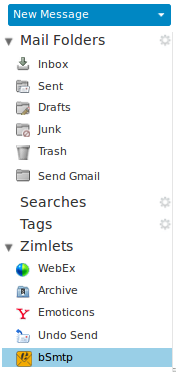
\includegraphics[clip,scale=0.45]{screenshots_user_en/Step1-1}
\par\end{centering}

\caption{\label{fig:Pas 1}Step \ref{enu:Pas 1} - Zimbra Sidebar \textrightarrow{}
Zimlets \textrightarrow{} \textbf{\emph{bSmtp}}}
\end{figure}


\item \label{enu:Pas 2}After opening settings, click\textbf{\emph{ Choose
the Folder}} (see figure \ref{fig:Pas 2}).


\begin{figure}[H]
\begin{centering}
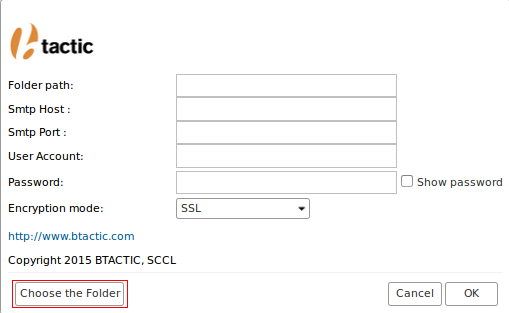
\includegraphics[clip,scale=0.45]{screenshots_user_en/Step1-2}
\par\end{centering}

\caption{\label{fig:Pas 2}Step \ref{enu:Pas 2} - Configuration bSmtp \textrightarrow{}
\textbf{\emph{Choose the Folder}}}
\end{figure}


\item \label{enu:Pas 3}Click\textbf{\emph{ New}} (see figure \ref{fig:Pas 3}).


\begin{figure}[H]
\begin{centering}
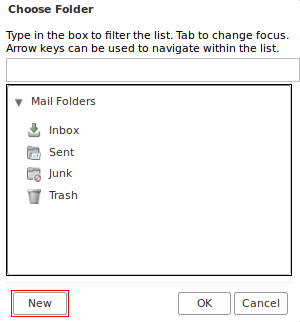
\includegraphics[clip,scale=0.45]{screenshots_user_en/Step1-3}
\par\end{centering}

\caption{\label{fig:Pas 3}Step \ref{enu:Pas 3} - Select the folder bSmtp
\textrightarrow{} \textbf{\emph{New}}}
\end{figure}


\item \label{enu:Pas 4}Specify which folder you want to send emails that
are stored by zimlet. It is advisable to choose a folder name or style
of Gmail Sent like. As can be seen in Figure \ref{fig:Pas 4}you must
specify the name of the folder in the \textbf{\emph{Name}} field and
then click\textbf{\emph{ OK}}.


\begin{figure}[H]
\begin{centering}
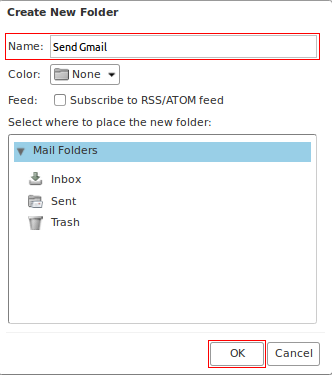
\includegraphics[clip,scale=0.44]{screenshots_user_en/Step1-4}
\par\end{centering}

\caption{\label{fig:Pas 4}Step \ref{enu:Pas 4} - Creation folder bSmtp}
\end{figure}


\item \label{enu:Pas 5}Select the folder you just created and click\textbf{\emph{
OK}} (see figure \ref{fig:Pas 5}).


\begin{figure}[H]
\begin{centering}
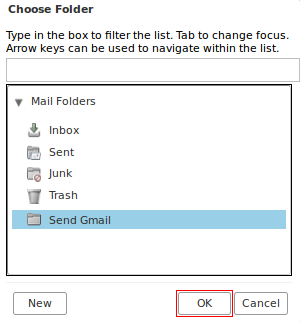
\includegraphics[clip,scale=0.44]{screenshots_user_en/Step1-5}
\par\end{centering}

\caption{\label{fig:Pas 5}Step \ref{enu:Pas 5} - Select the folder bSmtp
\textrightarrow{} \textbf{\emph{OK}}}
\end{figure}


\item \label{enu:Pas 6}Specify data email account you want to use to send
emails and finally click\textbf{\emph{ OK}} (see figure \ref{fig:Pas 6}).
You must specify all fields least \textbf{\emph{Folder path}} because
this field as we have configured following steps 2, 3, 4 and 5. If
you want to set up a Gmail see section \ref{sub:Configurar una Compta de Gmail}.


\begin{figure}[H]
\begin{centering}
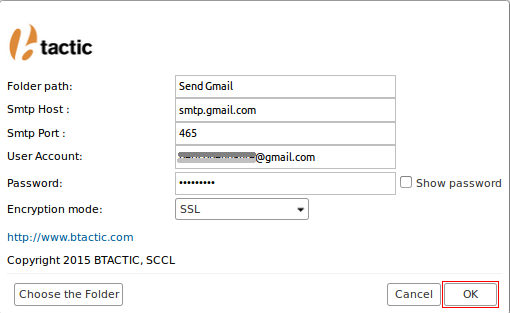
\includegraphics[clip,scale=0.45]{screenshots_user_en/Step1-6}
\par\end{centering}

\caption{\label{fig:Pas 6}Step \ref{enu:Pas 6} - Setting the email account
to use}
\end{figure}


\end{enumerate}
We have set up the email account and we can send mail from this account.


\subsection{Considerations}

Is if you want to change the email account to use the process must
be repeated by following steps \ref{enu:Pas 1} and \ref{enu:Pas 6}.
If we wanted to continue emails sent are stored in the same folder.
If you want to store in a different folder follow all the steps again.\\
\\
If the account password is changed external email they have to follow
steps \ref{enu:Pas 1} and \ref{enu:Pas 6}, Then you will need to
modify the password field, otherwise the zimlet not be able to make
deliveries.


\subsection{\label{sub:Configurar una Compta de Gmail}Set up a Gmail account}

If you want to use a Gmail account we must set Gmail account to allow
zimlet can send emails. Let the process to continue.\\
\\
The first wing must access Gmail account you want to use. Once we
have identified follow these steps:
\begin{enumerate}
\item \label{enu2:Pas 1}Access to\textbf{\emph{ My account}} (see figure
\ref{fig:Configurar Gmail - Pas 1}).


\begin{figure}[H]
\begin{centering}
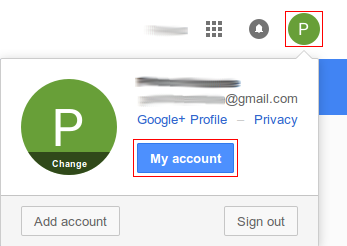
\includegraphics[clip,scale=0.45]{screenshots_user_en/Step2-1}
\par\end{centering}

\caption{\label{fig:Configurar Gmail - Pas 1}Step \ref{enu2:Pas 1} - Access
settings Gmail account}
\end{figure}


\item \label{enu2:Pas 2}Access to\textbf{\emph{ Connected apps }}\textbf{\&}\textbf{\emph{
sites}} (see figure \ref{fig:Configurar Gmail - Pas 2}).


\begin{figure}[H]
\begin{centering}
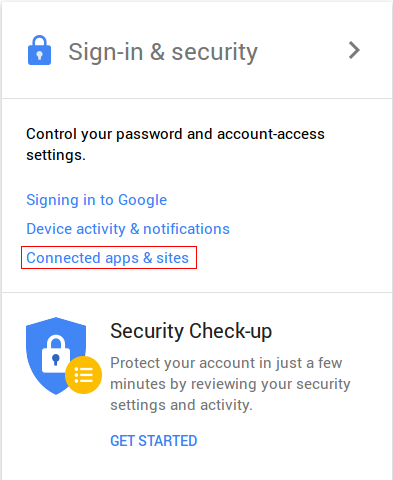
\includegraphics[clip,scale=0.45]{screenshots_user_en/Step2-2}
\par\end{centering}

\caption{\label{fig:Configurar Gmail - Pas 2}Step \ref{enu2:Pas 2} - Access
to Connected apps \& sites}
\end{figure}


\item \label{enu2:Pas 3}Active the option\textbf{\emph{ Allow less secure
apps}} (see figure \ref{fig:Configurar Gmail - Pas 3}).


\begin{figure}[H]
\begin{centering}
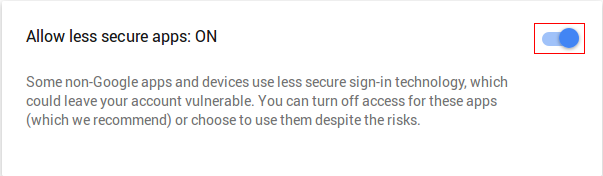
\includegraphics[clip,scale=0.45]{screenshots_user_en/Step2-3}
\par\end{centering}

\caption{\label{fig:Configurar Gmail - Pas 3}Step \ref{enu2:Pas 3} - Allow
less secure apps}
\end{figure}


\end{enumerate}
After editing permissions Gmail can now configure the zimlet following
the steps in \ref{sec:1 Configuraci=0000F3 inicial del Zimlet}. In
Step \ref{enu:Pas 6} we have to use these parameters::
\begin{itemize}
\item Host Smtp: smtp.gmail.com
\item Port Smtp: 465
\item User Account: <email address Gmail>
\item Password: <password Gmail account>
\item Encryption mode: SSL
\end{itemize}

\section{Using the zimlet}

To send an email from the account we have previously set up following
these steps:
\begin{enumerate}
\item \label{enu3:Pas 1}Compose an email in the usual way and once we have
it ready to be sent, instead of clicking \emph{Send} you have to click
\textbf{\emph{Send by SMTP}} (see figure \ref{fig:Enviar correu electr=0000F2nic}).
From now on we have two options when sending a mail::

\begin{itemize}
\item Click\textbf{\emph{ Send}}: mail will be sent from the account of
Zimbra.
\item Click\textbf{\emph{ Send by SMTP}}: mail will be sent from the external
account that you previously configured.
\end{itemize}

\begin{figure}[H]
\begin{centering}
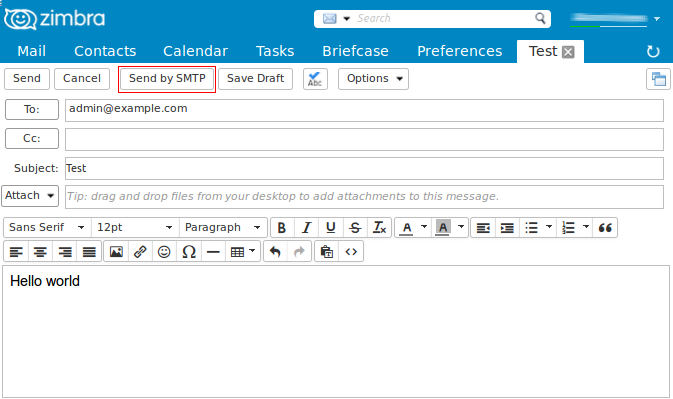
\includegraphics[clip,scale=0.45]{screenshots_user_en/Step3-1}
\par\end{centering}

\caption{\label{fig:Enviar correu electr=0000F2nic}Step \ref{enu3:Pas 1}
- Send email}
\end{figure}


\item \label{enu3:Pas 2}When sending mail may be that we display the message
in Figure \ref{fig:Confirmaci=0000F3 desar email}. In this case you
have to click on \textbf{\emph{Yes}}.


\begin{figure}[H]
\begin{centering}
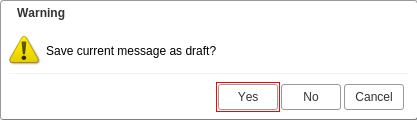
\includegraphics[clip,scale=0.45]{screenshots_user_en/Step3-2}
\par\end{centering}

\caption{\label{fig:Confirmaci=0000F3 desar email}Step \ref{enu3:Pas 2} -
Confirmation email store}
\end{figure}


\item \label{enu3:Pas 3}Finally, the email will be stored in the folder
you have specified (see figure \ref{fig:Enviados}).


\begin{figure}[H]
\begin{centering}
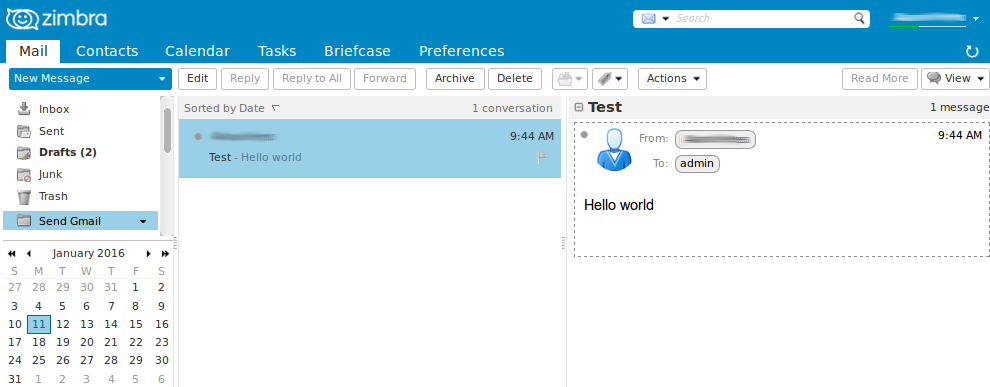
\includegraphics[clip,scale=0.45]{screenshots_user_en/Step3-3}
\par\end{centering}

\caption{\label{fig:Enviados}Step \ref{enu3:Pas 3} - Folder Email sent from
zimlet}
\end{figure}
\end{enumerate}

\end{document}
